\section{Problem description}
\label{sec:Problem description}
In this section, we first introduce the basic concepts needed in this paper, then present our survivable virtual network embedding problem.




% $F^S$ is the function type set $F^S_i$ on which every substrate node can execute, $F^S_i$ is consisted from different function type $f_j$. Each substrate node (link) is associated with the residual computing (communication) resource capacity. Each node $v_i$ has an available computational capacity of $c_i$. The node number of substrate nodes is $m$. Each undirected link $e_{ij}$ has an available bandwidth of $b_{ij}$. The number of function type is $p$. In Fig.\ref{fig:VNmapSN} (a) substrate network, substrate nodes set $V^S$ is $\{s_1,s_2,s_3,s_4,s_5,s_6,s_7\}$, substrate edges set $E^S$ is $\{s_1s_2,s_1s_3,s_1s_4,s_1s_5,s_2s_3,s_2s_5,s_3s_5,s_3s_6,s_3s_7,s_4s_7\}$ substrate nodes's function type set $F^S$ is $\{\{f_1\},\{f_2,f_3\},\{f_3\},\{f_4\},\{f_1,f_2\},\{f_1,f_4\},\{f_2,f_3\}\}$.

\subsection{Virtual Network}
We represent a virtual network (VN) as an undirected graph $G (V,E)$ where $V$ and  $E$ are the sets of virtual nodes and virtual links, respectively. Each virtual link $e_{ij}$ has the bandwidth demand $d_{ij}$. Each virtual node (i.e, $v_i$) has a computation resource demand $d_i$. For virtual node $v_i$, the virtual function executed on the virtual node is denoted as $f(i)$. As shown in Fig.\ref{fig:VNQSNVNE}(A), virtual nodes set $V$ is $\{v_1,v_2,v_3,v_4\}$, virtual edges set $E$ is $\{e_{12},e_{13},e_{14},e_{23}\}$, virtual nodes executing function $f(i)$ is $\{f_1,f_2,f_3,f_4\}$.

\begin{figure*}
\centering
% Requires \usepackage{graphicx}
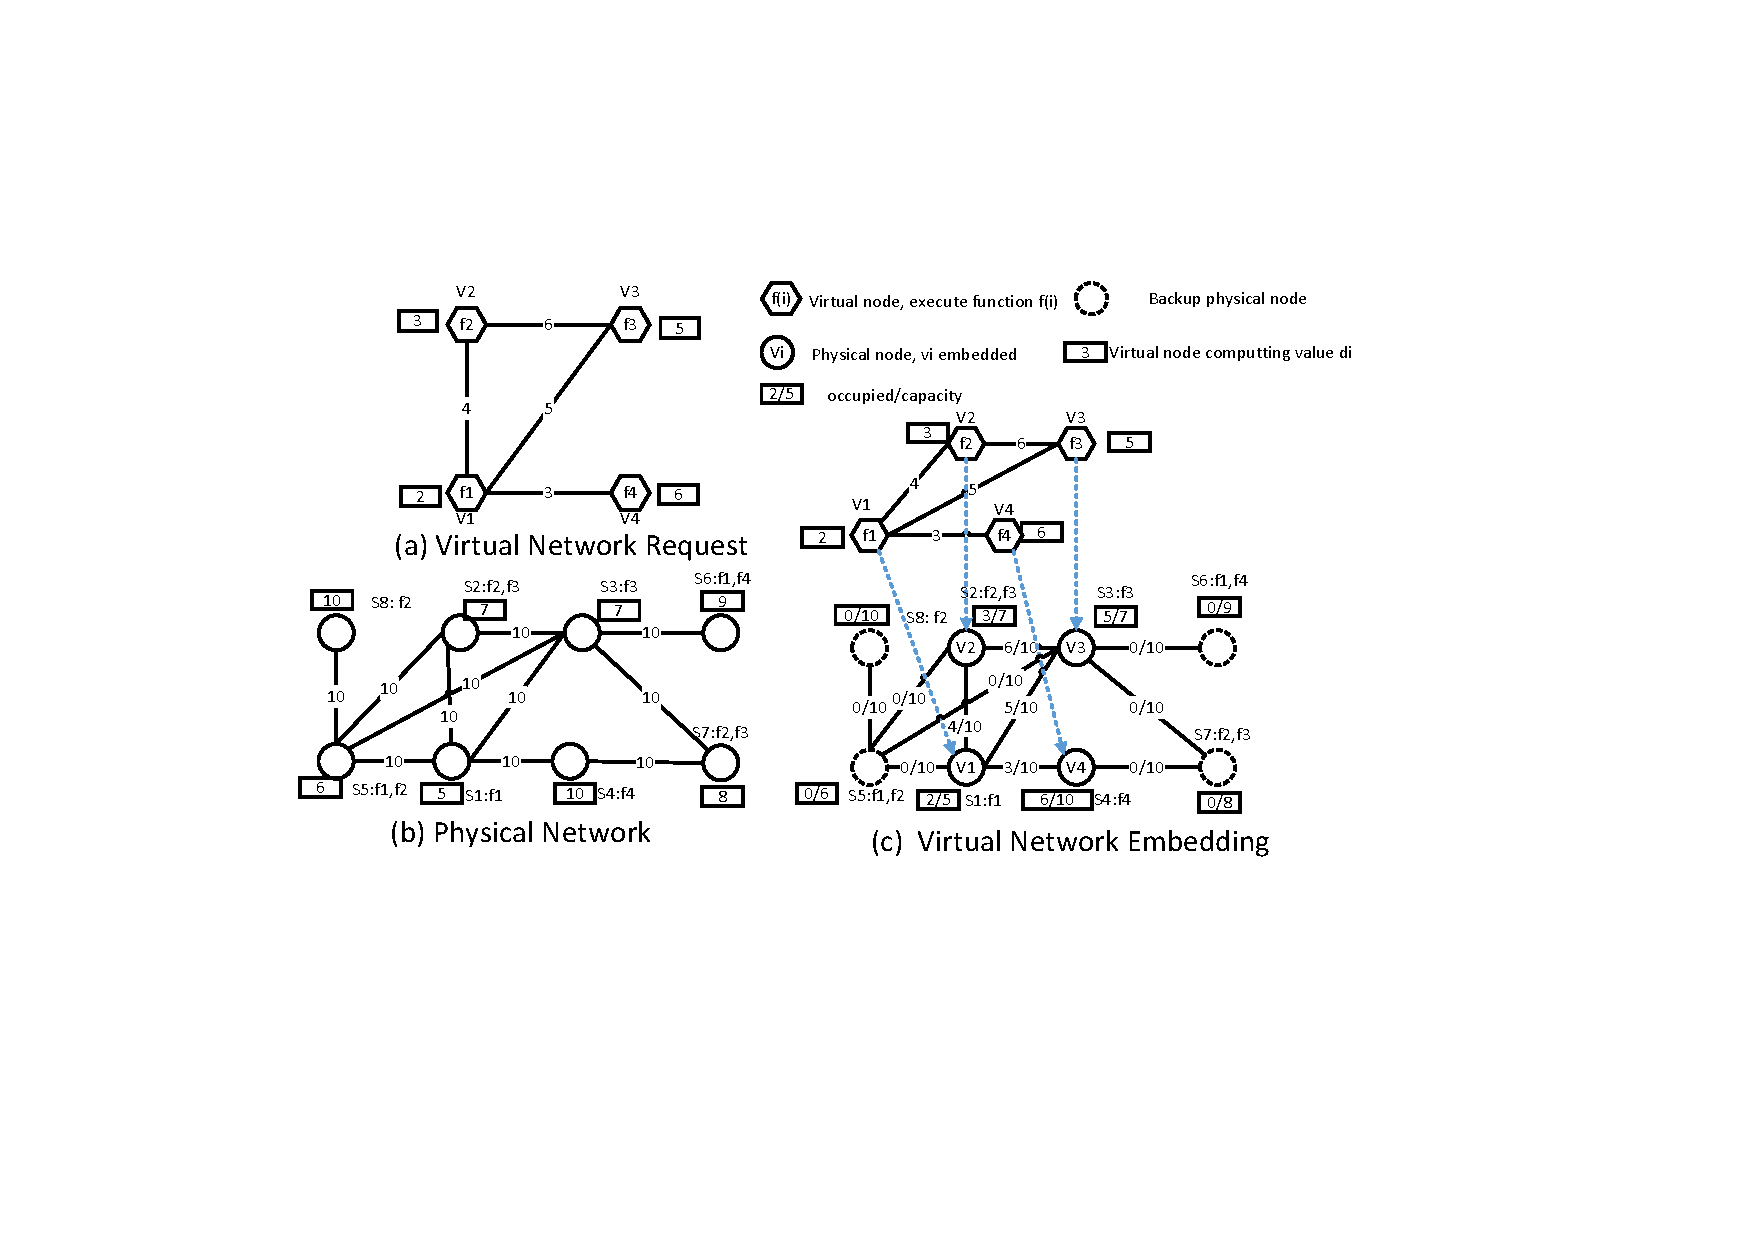
\includegraphics[width=5in]{Fig/VNQSNVNE}\\
\caption{(A) Virtual Network Request $G(V,E)$, $V=\{v_1,v_2,v_3,v_4\}$, $E=\{e_{12},e_{23},e_{13},e_{14}\}$,  $f(i)=\{f_1,f_2,f_3,f_4\}$, $d_i=\{2,3,5,6\}$, $d_{ij}=\{4,5,3,6\}.$(B) Physical Network $G^S(S,L), S=\{s_1,s_2,s_3,s_4,s_5,s_6,s_7,s_8\}, L=\{l_{12},l_{13},l_{14},l_{15},l_{23},l_{25},l_{35},l_{36},l_{37},l_{47},l_{58}\}, F(i)=\{\{f_1\},\{f_2,f_3\},\{f_3\},\{f_4\},\{f_1,f_2\},\{f_1,f_4\},\{f_2,f_3\}\}, c_i=\{5,7,7,10,6,9,8,10\}, b_{ij}=\{10,10,10,10,10,10,10,10,10,10,10\}$ (C)}\label{fig:VNQSNVNE}
\end{figure*}

%\begin{figure}
%\centering
%\begin{minipage}[t]{0.45\linewidth}
%% Requires \usepackage{graphicx}
%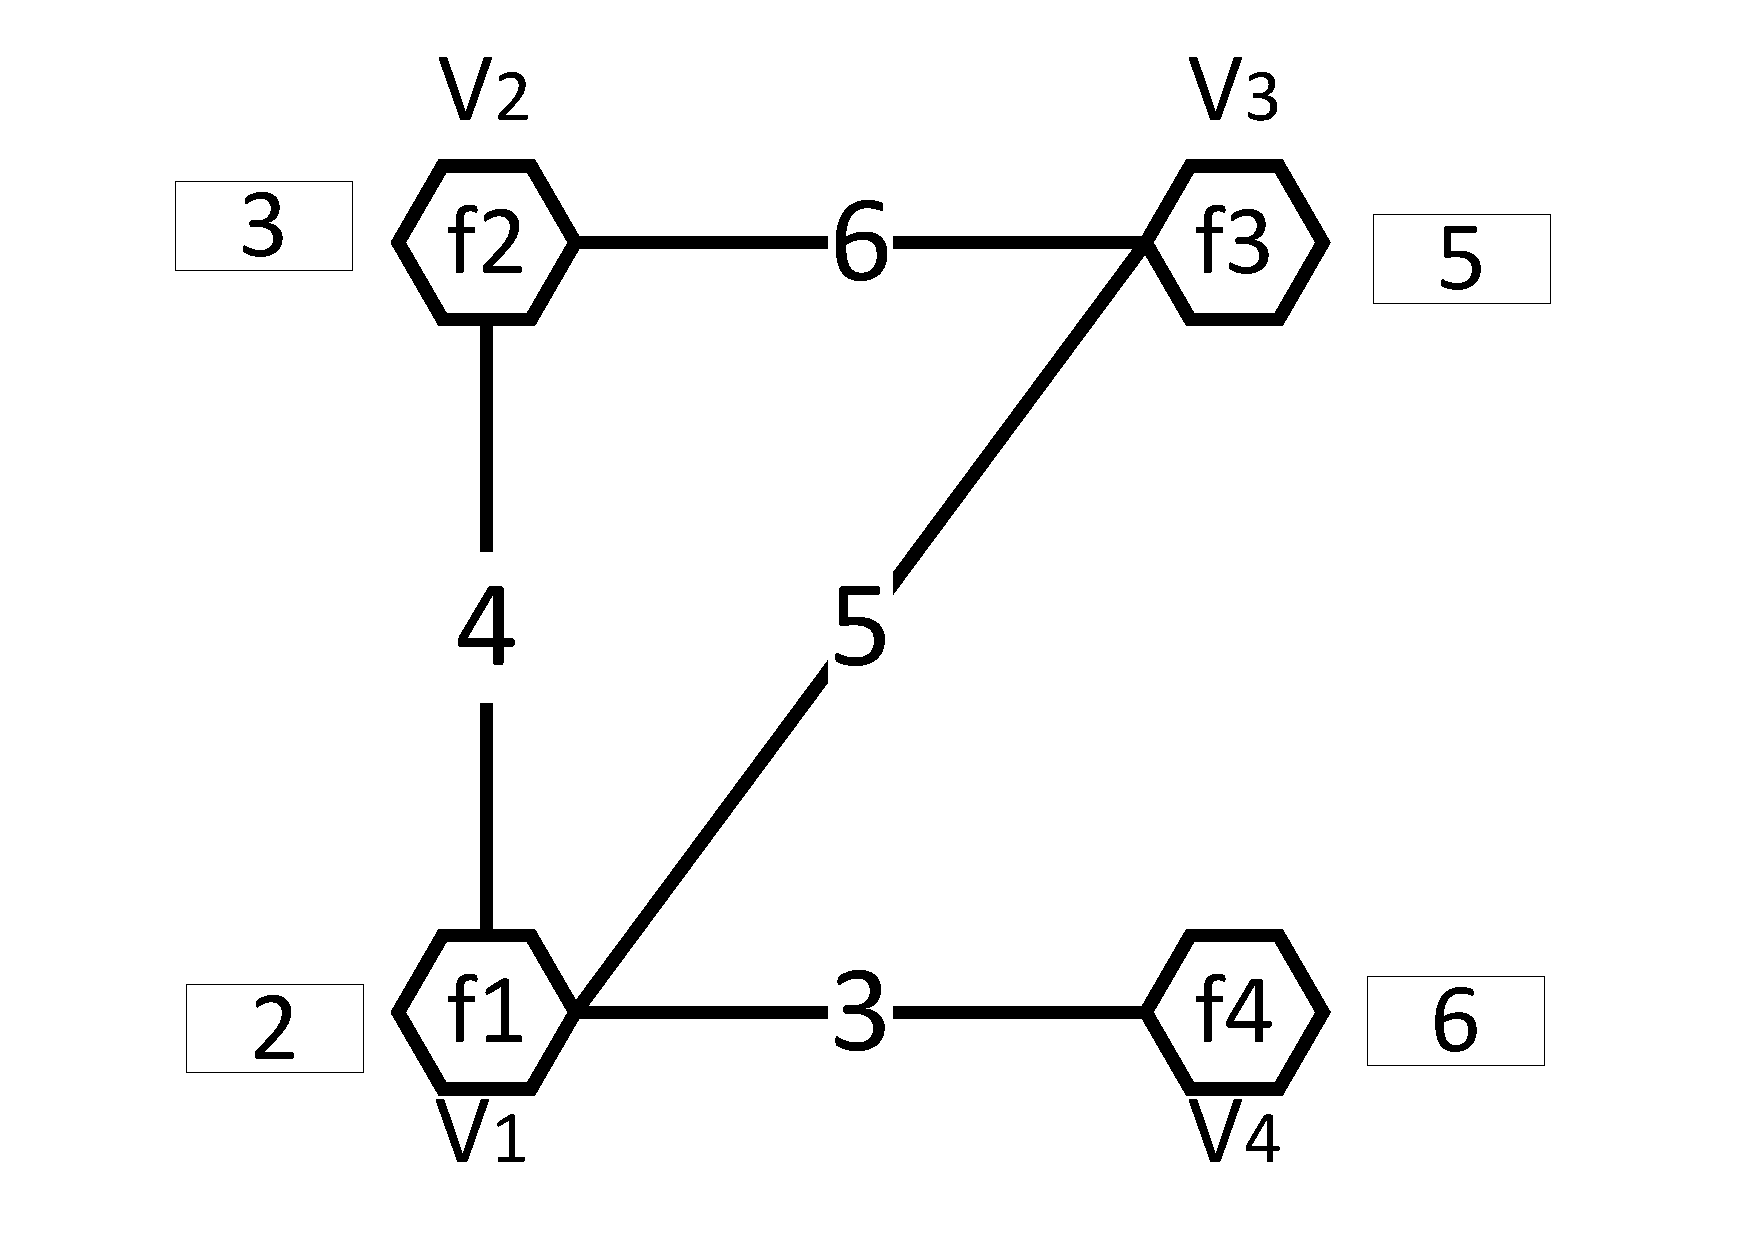
\includegraphics[width=1.3in]{Fig/VNQ}\\
%\caption{Virtual Network Request $G(V,E)$, $V=\{v_1,v_2,v_3,v_4\}$, $E=\{e_{12},e_{23},e_{13},e_{14}\}$,  $f(i)=\{f_1,f_2,f_3,f_4\}$, $d_i=\{2,3,5,6\}$, $d_{ij}=\{4,5,3,6\}.$}\label{fig:VNQ}
%\end{minipage}
%\hfill
%\begin{minipage}[t]{0.45\linewidth}
%% Requires \usepackage{graphicx}
%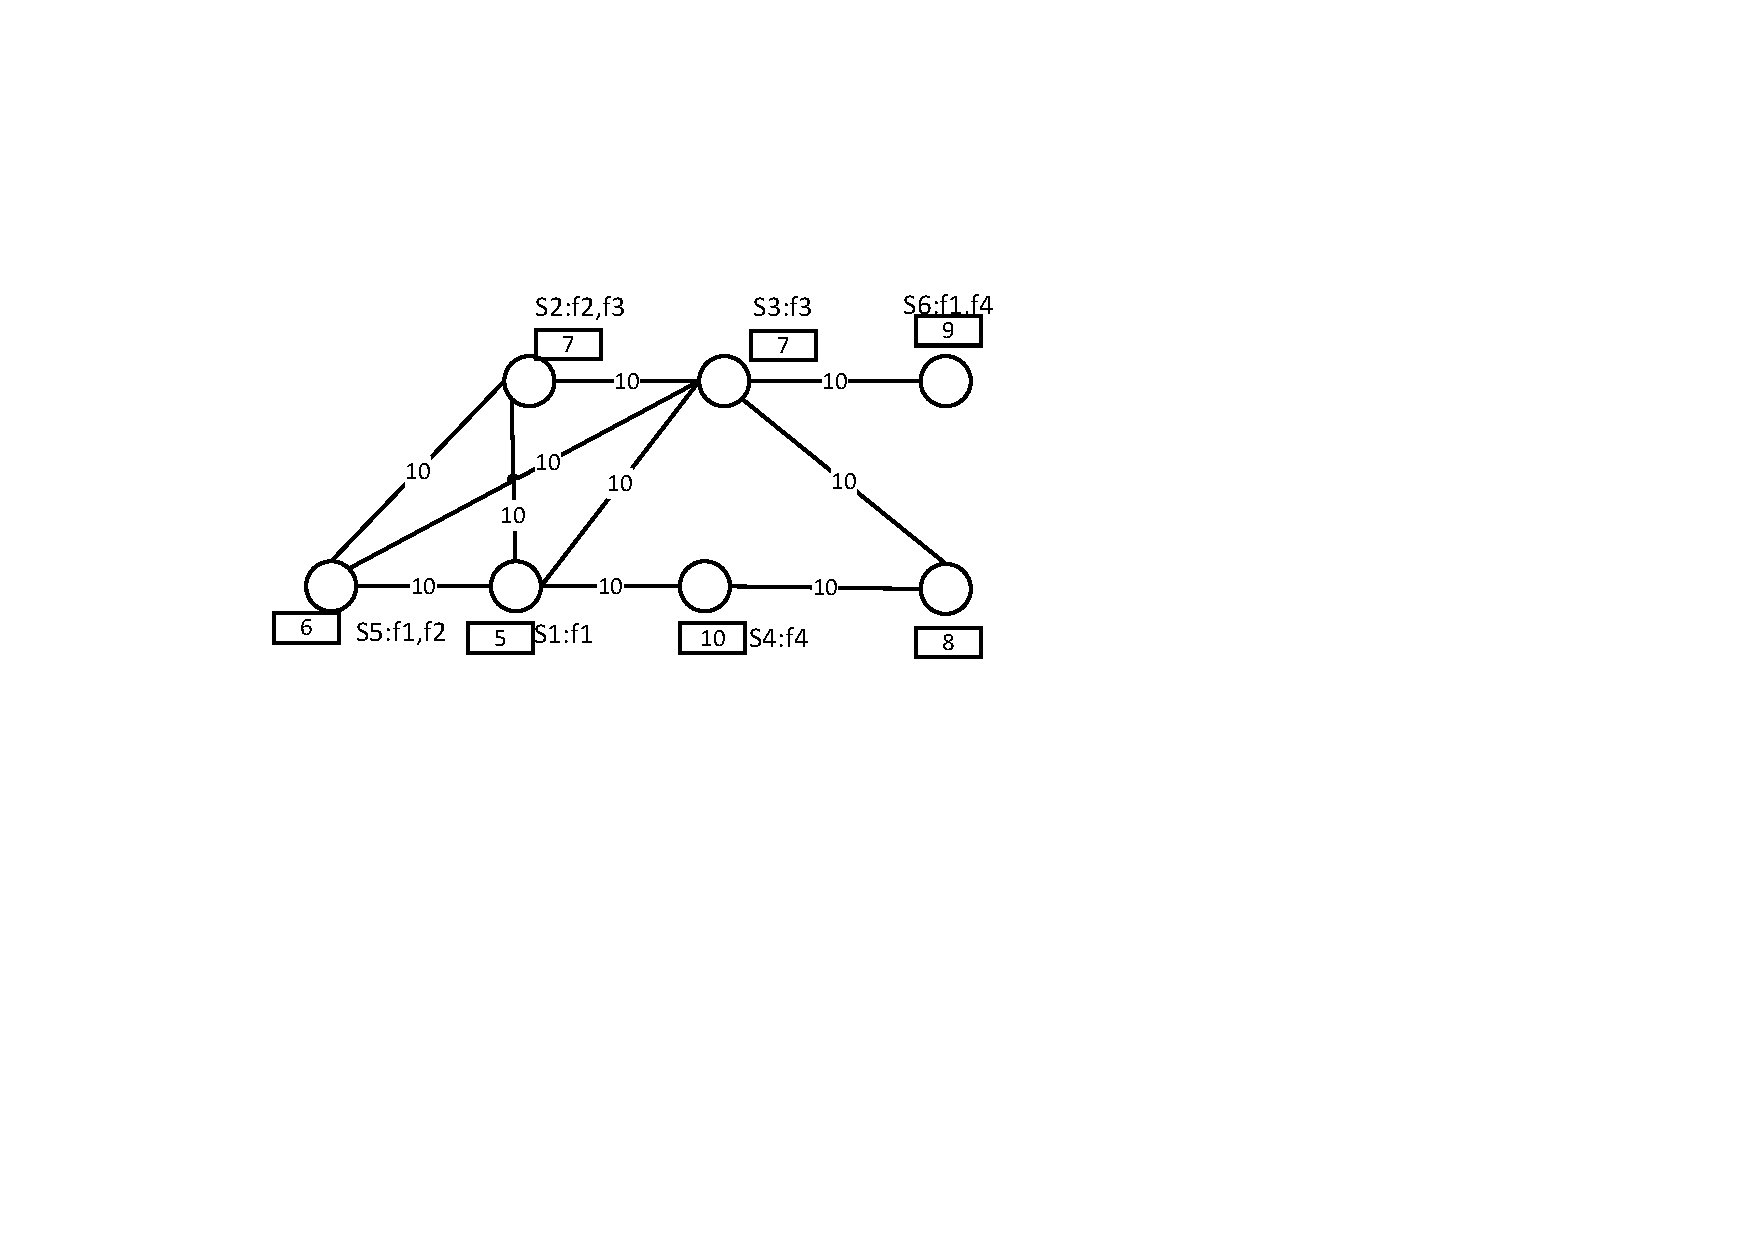
\includegraphics[width=1.8in]{Fig/SN}\\
%\caption{Physical Network $G^S(S,L), S=\{s_1,s_2,s_3,s_4,s_5,s_6,s_7\}, L=\{l_{12},l_{13},l_{14},l_{15},l_{23},l_{25},l_{35},l_{36},l_{37},l_{47}\}, F(i)=\{\{f_1\},\{f_2,f_3\},\{f_3\},\{f_4\},\{f_1,f_2\},\{f_1,f_4\},\{f_2,f_3\}\}, c_i=\{5,7,7,10,6,9,8\}, b_{ij}=\{10,10,10,10,10,10,10,10,10,10\}$}\label{fig:SN}
%\end{minipage}
%\end{figure}

\subsection{Physical Network}
We model the physical network as an undirected graph $G (S,L)$, where $S$ and $L$ is the sets of physical nodes and physical links, respectively. For physical node $s_i$, $F(i)$ is the set of virtual functions can executed on this  node, $c_i$ is the available computational capacity. Each physical link $l_{ij}$ has an available bandwidth of $b_{ij}$. In Fig.\ref{fig:VNQSNVNE}(B) physical network, physical nodes set $S$ is $\{s_1,s_2,s_3,s_4,s_5,s_6,s_7\}$,  links set $L$ is $\{l_{12},l_{13},l_{14},l_{15},l_{23},l_{25},l_{35},l_{36},l_{37},l_{47}\}$, substrate nodes's function type set $F(i)$ is $\{\{f_1\},\{f_2,f_3\},\{f_3\},\{f_4\},\{f_1,f_2\},\{f_1,f_4\},\{f_2,f_3\}\}$.



\subsection{Virtual Network Embedding}
Given the VN request $G (V,E)$, the problem of virtual network embedding aims to map this request onto the physical network $G^S (S,L)$ while providing enough resource as demanded.
To satisfy the request from both virtual node and virtual links, virtual network embedding  can be divided in two sub-problems:

Virtual Node Mapping (VNoM) where virtual nodes $v_i$ have to be allocated in physical nodes $s_j$, and computation resource demand $d_i$ of virtual nodes $v_i$ do not more than available computational capacity $c_j$ of physical network.

Virtual Link Mapping (VLiM) where virtual links $e_{ij}$ connecting these virtual nodes have to be mapped to paths connecting the corresponding nodes in the substrate network,  .....

Besides nodes and link constraints, there is a location constraint, that is, a virtual node ${v_i} \in V$ can only be provisioned on a physical node $s_j$ with ${f_i} \in {F_j}$. That is, the virtual function running on virtual node ${v_i}$ can be executed on physical node $s_j$.

As shown in Fig.\ref{fig:VNQSNVNE}(C), we embed virtual network request as shown in Fig.\ref{fig:VNQSNVNE}(A) into the substrate network, node $v_1$ is embedded in node $s_1$, node $v_2$ is embedded in node $s_2$, node $v_3$ is embedded in node $s_3$, node $v_4$ is embedded in node $s_4$. demand node computing of every virtual node is not more than these virtual nodes corresponding substrate node's remain node computing. Every link of virtual network request exist a corresponding path consisted of substrate node and remain bandwidth of all links of corresponding path is more than demand  bandwidth of the virtual network link.


Lots of studies investigate the virtual network embedding problem \cite{lischka2009virtual}, as the focus of this paper is not virtual network embedding, we adopt algorithm in [lischka2009virtual] as the basic virtual network embedding algorithm.
There has existed most studies about virtual network embedding method listed in a survey paper\cite{fischer2013virtual}.


\subsection{Node Failure}
Due to malicious attacks, natural disasters, unintentional cable cuts, planned maintenance, equipment malfunctioning, physical nodes that host the virtual nodes may suffer unavoidable fail. Failure in the VN can happen when single or multiple network components failures, which results in financial losses. In general, the multiple physical node's simultaneous failure is mutual independent, a single node failure happen at most of time\cite{yeow2011designing}. In this paper, we study the survivable virtual network embedding problem with single node failure. In section, we will discuss how our algorithm can be extended to the scenario with multiple node failure.


Node failures not only effect the virtualized services running on the failed server, but also would terminate all the communications which traverse through this node. To handle single node failure, one straightforward way  is to provision dedicated backup resource for each virtual node and virtual link in a VN request, also known as the 1 + 1-protection scheme. Fig.\ref{fig:FI} utilize an example to illustrate this straightforward way. There are totally 5 virtual nodes and 4 virtual links. To provide 1 + 1-protection scheme,  4 backup nodes, 8 backup links are added in the graph. For example, when node $s_2$ fails, as it runs function $f_2$ for $v_2$ in the VN network, one backup node $s_8$ with $F(8)=f_2$ and two backup links $(s_8, s_1)$ and $(s_8, s_3)$ are added. However, large amount of  resource are needed to add under this straightforward way.

To minimize the additional resources needed, this paper solve following survivable virtual network embedding problem: when single node fails

Given a NV request $G(V,E)$ and its embedding , computer the  minimum additional resources

Given a NV request $G(V,E)$, for each node $v_i$, denote its attached physical node as $a(v_i)$. The node resource for virtual network embeddi



On the one hand, node failures  directly. On the other hand, a failure of a physical node

 two
 Survivability is the ability of a system such as a computer or a communication network to operate correctly in the presence of faults. From these studies, we can conclude that .




Given

 One extreme case for the VN protection approach
physical node may suffer the problem of instance fail.


Given the present-day importance of communications systems and infrastructures in general, networks should be designed and operated in such a way that failures can be mitigated. Network nodes  might for instance fail , and so forth. Survivable have been used by the networking community to capture the ability of a communications system to maintain operation when confronted
with network failures.

Therefore, in this paper, we just design a single node failure situation, but we will discuss that our algorithm extend for adapting multiple node failure situation.


\subsection{Survivable}
%We define reliability as the probability that critical nodes of a VInf remain in operation, over all possible node failures. This is not to be confused with availability, which is defined as a ratio of uptime to the sum of uptime and downtime

Survivability is guaranteed on the set of critical nodes of a VN through redundant virtual nodes with backup nodes set $B(V,F)$, we suppose all virtual node as critical node in this paper. In Fig.\ref{fig:eVN}, node set $V$ of backup node $B(V,S)$ is $\{s_5,s_6,s_7\}$, function type set $F$ of node is $\{\{f_1,f_2\},\{f_1,f_4\},\{f_2,f_3\}\}$. A backup (redundant) node $b_i$ may not be able to assume full execution function of a failed critical node. Hence, the backup node may not have sufficient resources in terms of computation resource.


%\subsection{How many backups?}
%The number of backup nodes depend on the physical mapping, and the failure models of both the physical nodes and the virtual infrastructure.

%The problem is to  allocate least resources for a VN $G$, including redundancy such that a reliability guarantee of at least r is achieved.


\subsection{Survivable embedded Virtual Network Request}

In this subsection, we define the SeVN design problem as follows, for a given VN request with $|V|$ nodes, the VN had been already embedded in substrate network SN and every node running function $f_i(f_i\in F^V_i)$, protect the VN with some augmented backup nodes and a set of appropriate links to connect these virtual nodes, and reserve sufficient computing and communication resources in these nodes and links to guarantee the restorability of VN request after a facility/substrate node failure.

There are different combinations of function type with respect to  every nodes of embedded virtual network, but there is only one type of function type running onto substrate node which corresponding one embedded virtual node at one moment.

There exist many backup virtual nodes $B(V,S)$ which are abstracted from un-startup substrate network's node. When one fault node $v_i$ appeared in virtual network request $G^V (V^V,E^V,f^V,C^V,B^V)$, Solving the survivable request of embedded virtual network is of approximately equivalence with asking 1-FNFT$(G,B)$ of graph $G$ and backup nodes set $B$ without computation and bandwidth's limitation.

There exist popular and easy to understand method\cite{yeow2011designing} as show in Fig.\ref{fig:FI}, when every virtual nodes fail iteratively because the corresponding the failure substrate node occur failure, then directly startup new node, connect link among nodes $V\cup B$, augment node computing or augment demand bandwidth of existing link as shown in \ref{fig:FI}. The rude method demand startup 4 new nodes, 8 new edges, 16 node computing and 36 edge bandwidth.

After a failure, even an unaffected virtual node may be migrated from a working host node to its corresponding backup host node, the former method\cite{yeow2011designing} do not consider the situation of node's migration.


We supposed a novel method STAR algorithm, which augment resource as shown in Fig.\ref{fig:FD}, our method demand startup 2 new nodes, 5 new edges, 11 node computing and 23 edge bandwidth.

\begin{figure}
\centering
\begin{minipage}[t]{0.4\linewidth}
\centering
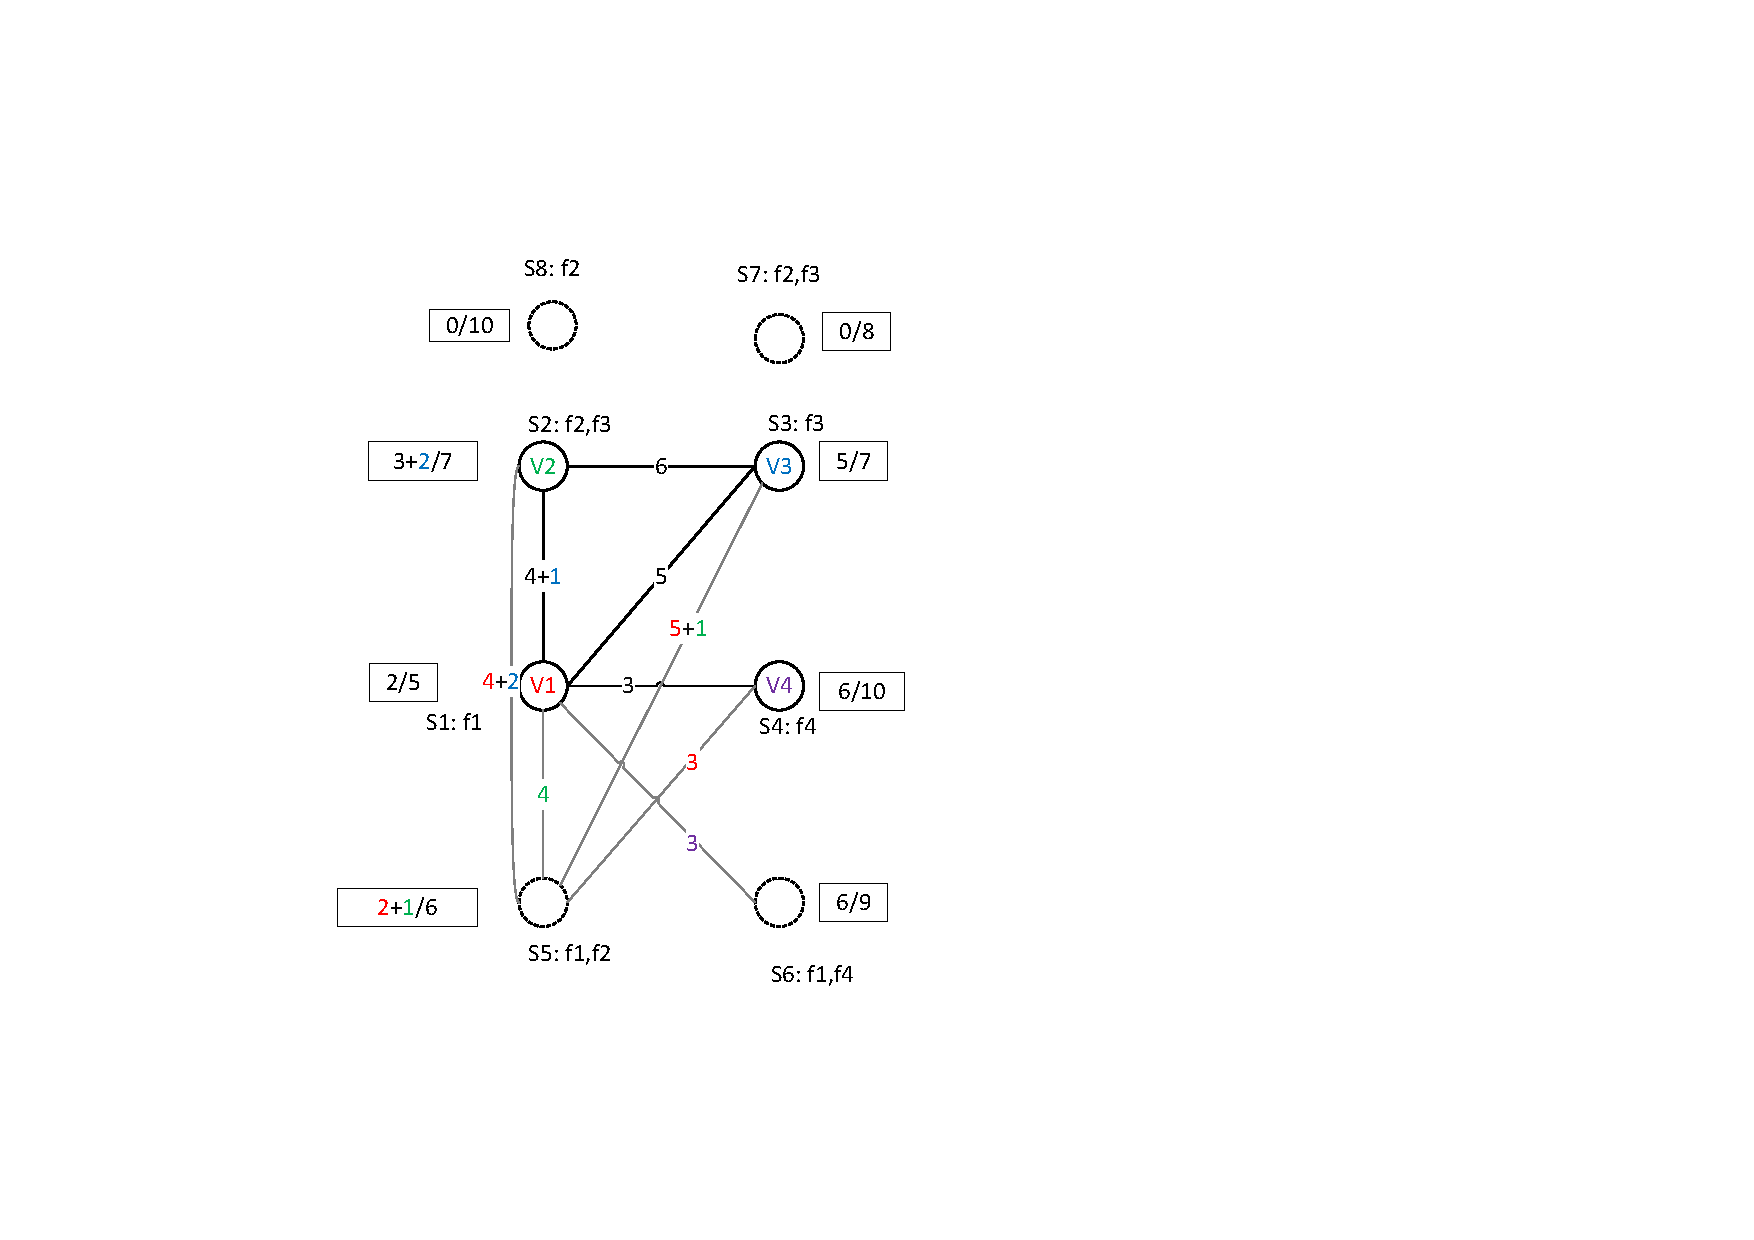
\includegraphics[width=1.5in]{Fig/FD}\\
\caption{ FD}\label{fig:FD}
\end{minipage}
\hfill
\begin{minipage}[t]{0.4\linewidth}
\centering
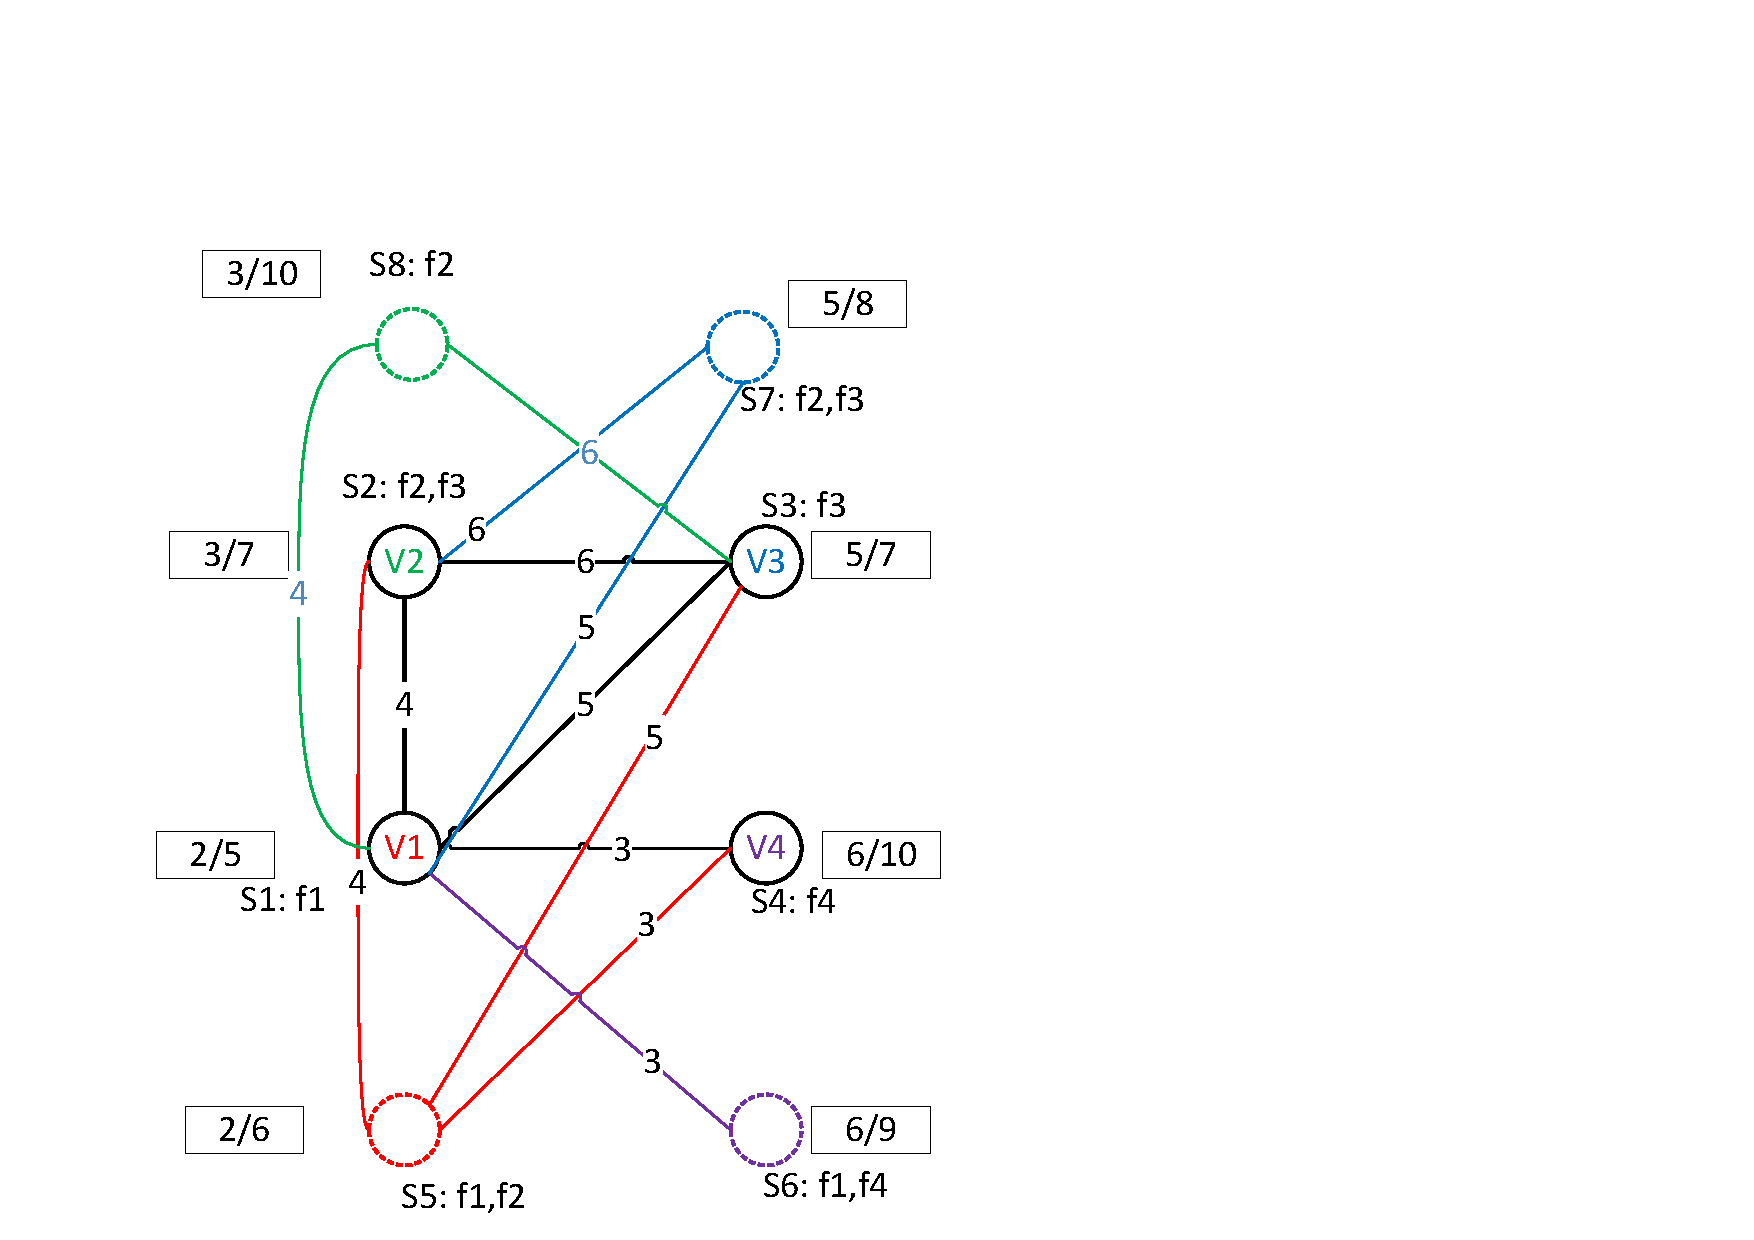
\includegraphics[width=1.5in]{Fig/FI}\\
\caption{FI}\label{fig:FI}
\end{minipage}
\end{figure}




There exist many approaches is modeled as the VN embedding (VNE) problem which attracts a broad interest recently\cite{fischer2013virtual}. VNE is extremely important in order to maximize the number of coexisting VNs and increase the utilization of substrate infrastructures. Virtual Network Embedding deals with the allocation of virtual resources both in nodes and links. Therefore, it can be divided in two sub-problems: Virtual Node Mapping (VNoM) where virtual nodes have to be allocated in physical nodes and Virtual Link Mapping (VLiM) where virtual links connecting these virtual nodes have to be mapped to paths connecting the
corresponding nodes in the substrate network. There has existed most studies about virtual network embedding method listed in a survey paper\cite{fischer2013virtual}. After all, we randomly choose a virtual network embedding method with considering three constraints: node computing, edge bandwidth and node function type from existed virtual network embedding method. As shown in Fig.\ref{fig:VNmapSN}(a), we embed virtual network request as shown in Fig.\ref{fig:VNQ} into the substrate network, node $v_1$ is embedded in node $s_1$, node $v_2$ is embedded in node $s_2$, node $v_3$ is embedded in node $s_3$, node $v_4$ is embedded in node $s_4$. demand node computing of every virtual node is not more than these virtual nodes corresponding substrate node's remain node computing. Every link of virtual network request exist a corresponding path consisted of substrate node and remain bandwidth of all links of corresponding path is more than demand  bandwidth of the virtual network link.


\subsection{Embedded Virtual Network}
\label{sec:embeddedVirtualNetwork}
When a virtual network request has been inserted in to substrate network, augmented resource is attached into virtual network, embedded virtual network denote as $G^V (V^V,E^V,f^V,F^V,C^V,B^V,M^V)$ as shown in Fig.\ref{fig:eVN}. $F^V$ denote a set of function type set $F^V_i$($f^V_i\in F^V_i$) which corresponding to every VN nodes $v_i$. $C^V$ denote node's computational resource's capacity. $B^V$ denote edge's bandwidth resource's capacity. $M^V$ denote node's mapping relationship of virtual network embedding algorithm, $M_{i}=j$ represent that the i-th VN's node had been embedded at j-th substrate network node. Besides, with respect to the node embedding, we suppose a assumption that all virtual nodes of VN should be mapped on isolated physically substrate nodes.
\begin{figure}
\centering
% Requires \usepackage{graphicx}
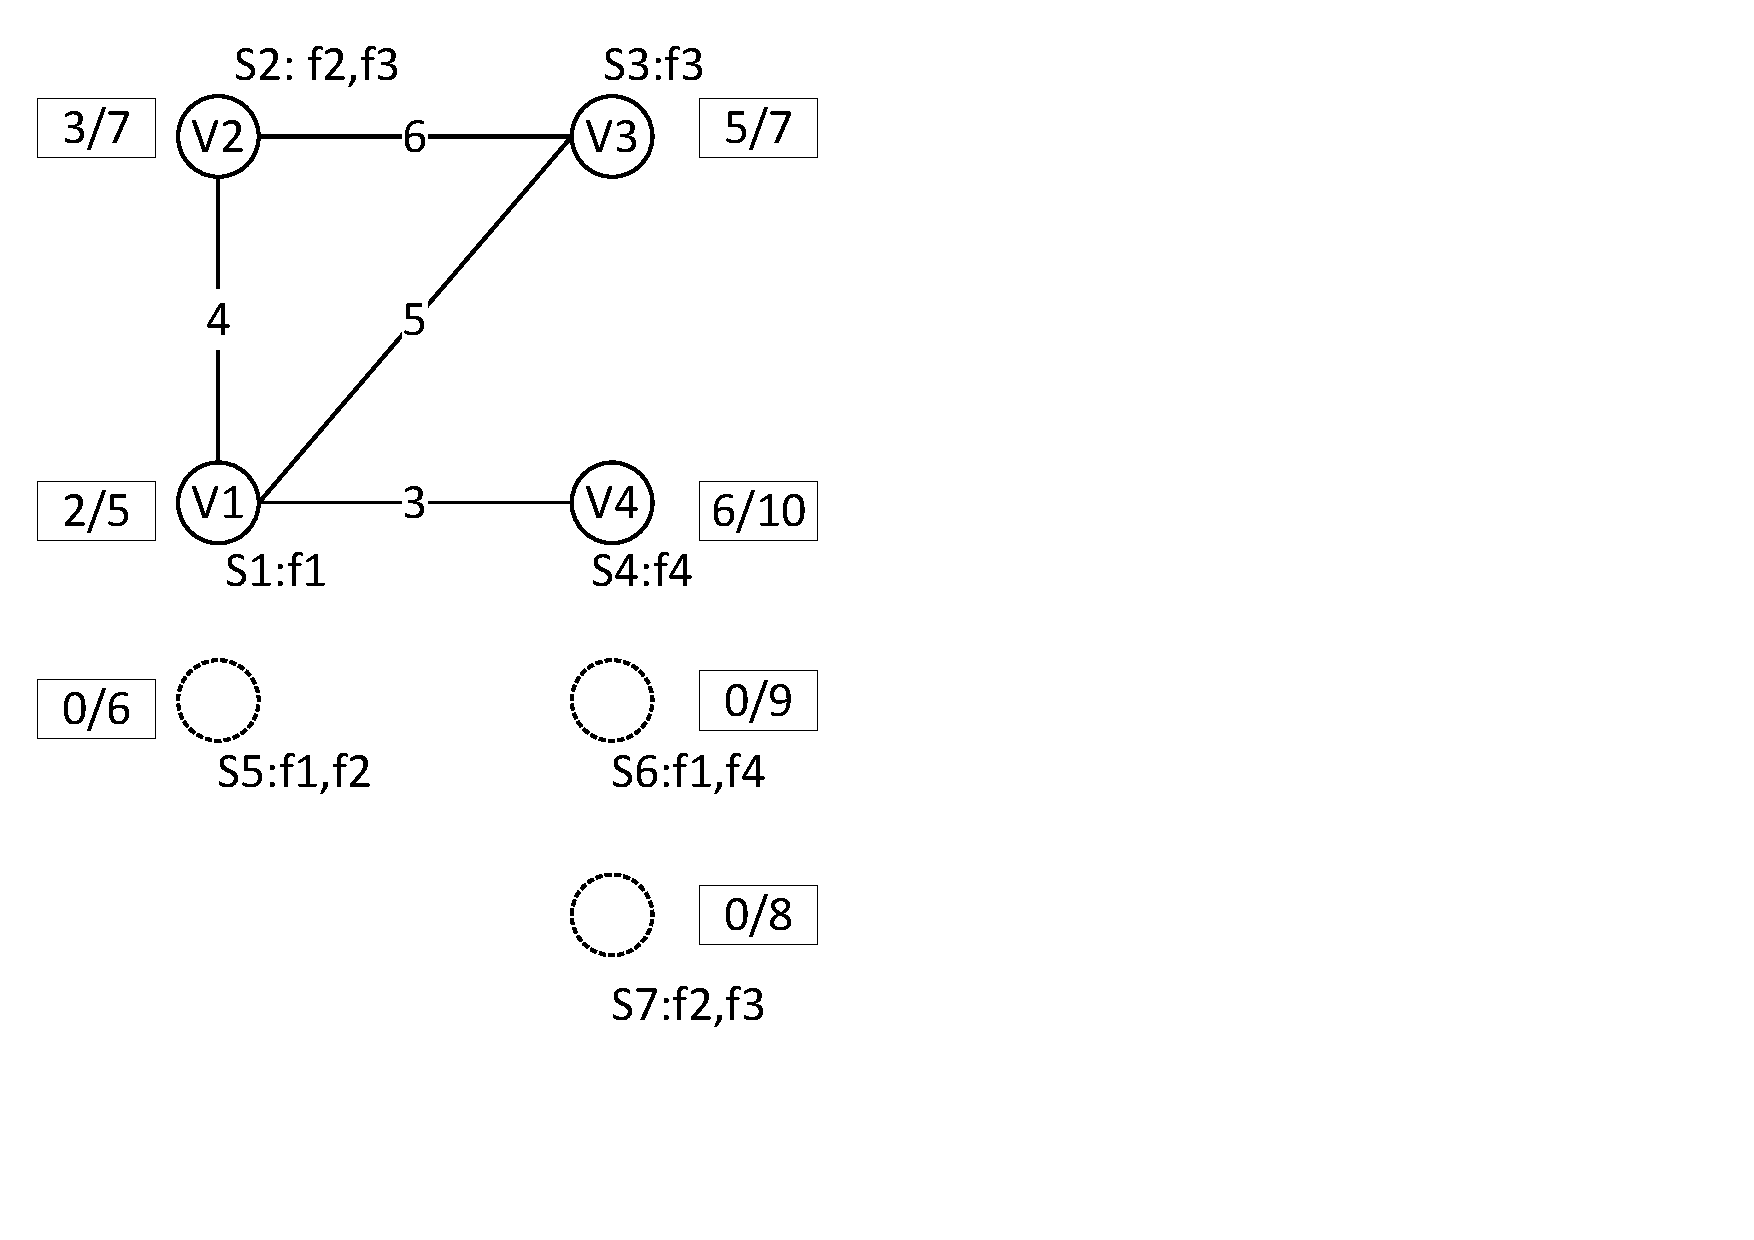
\includegraphics[width=2in]{Fig/eVN}\\
\caption{embedded Virtual Network $G^V (V^V,E^V,f^V,F^V,C^V,B^V,M^V_V)$, $V^V:\{s_1,s_2,s_3,s_4,s_5,s_6,s_7\}$, $E^V=\{e_{12},e_{23},e_{13},e_{14}\}$, $f^V:\{f_1,f_2,f_3,f_4\}$,
$F^V=\{\{f_1\},\{f_2,f_3\},\{f_3\},\{f_4\},\{f_1,f_2\},\{f_1,f_4\},\{f_2,f_3\}\}$, $C^V=\{5,7,7,10,6,9,8\}$, $B^V=\{4,6,5,3\}$, $M^V=\{s_1,s_2,s_3,s_4\}$}\label{fig:eVN}
\end{figure}


\subsection{Node Failure}
Given the present-day importance of communications systems and infrastructures in general, networks should be designed and operated in such a way that failures can be mitigated. Network nodes  might for instance fail due to malicious attacks, natural disasters, unintentional cable cuts, planned maintenance, equipment malfunctioning, and so forth. Survivable have been used by the networking community to capture the ability of a communications system to maintain operation when confronted
with network failures.

In general, the substrate nodes simultaneous failure is mutual independent , a single node failure happen at most of time\cite{yeow2011designing}. Therefore, in this paper, we just design a single node failure situation, but we will discuss that our algorithm extend for adapting multiple node failure situation.


\subsection{Survivable}
%We define reliability as the probability that critical nodes of a VInf remain in operation, over all possible node failures. This is not to be confused with availability, which is defined as a ratio of uptime to the sum of uptime and downtime

Survivability is guaranteed on the set of critical nodes of a VN through redundant virtual nodes with backup nodes set $B(V,F)$, we suppose all virtual node as critical node in this paper. In Fig.\ref{fig:eVN}, node set $V$ of backup node $B(V,S)$ is $\{s_5,s_6,s_7\}$, function type set $F$ of node is $\{\{f_1,f_2\},\{f_1,f_4\},\{f_2,f_3\}\}$. A backup (redundant) node $b_i$ may not be able to assume full execution function of a failed critical node. Hence, the backup node may not have sufficient resources in terms of computation resource.


%\subsection{How many backups?}
%The number of backup nodes depend on the physical mapping, and the failure models of both the physical nodes and the virtual infrastructure.

%The problem is to  allocate least resources for a VN $G$, including redundancy such that a reliability guarantee of at least r is achieved.


\subsection{Survivable embedded Virtual Network Request}

In this subsection, we define the SeVN design problem as follows, for a given VN request with $|V|$ nodes, the VN had been already embedded in substrate network SN and every node running function $f_i(f_i\in F^V_i)$, protect the VN with some augmented backup nodes and a set of appropriate links to connect these virtual nodes, and reserve sufficient computing and communication resources in these nodes and links to guarantee the restorability of VN request after a facility/substrate node failure.

There are different combinations of function type with respect to  every nodes of embedded virtual network, but there is only one type of function type running onto substrate node which corresponding one embedded virtual node at one moment.

There exist many backup virtual nodes $B(V,S)$ which are abstracted from un-startup substrate network's node. When one fault node $v_i$ appeared in virtual network request $G^V (V^V,E^V,f^V,C^V,B^V)$, Solving the survivable request of embedded virtual network is of approximately equivalence with asking 1-FNFT$(G,B)$ of graph $G$ and backup nodes set $B$ without computation and bandwidth's limitation.

There exist popular and easy to understand method\cite{yeow2011designing} as show in Fig.\ref{fig:FI}, when every virtual nodes fail iteratively because the corresponding the failure substrate node occur failure, then directly startup new node, connect link among nodes $V\cup B$, augment node computing or augment demand bandwidth of existing link as shown in \ref{fig:FI}. The rude method demand startup 4 new nodes, 8 new edges, 16 node computing and 36 edge bandwidth.

After a failure, even an unaffected virtual node may be migrated from a working host node to its corresponding backup host node, the former method\cite{yeow2011designing} do not consider the situation of node's migration.


We supposed a novel method STAR algorithm, which augment resource as shown in Fig.\ref{fig:FD}, our method demand startup 2 new nodes, 5 new edges, 11 node computing and 23 edge bandwidth.

\begin{figure}
\centering
\begin{minipage}[t]{0.4\linewidth}
\centering
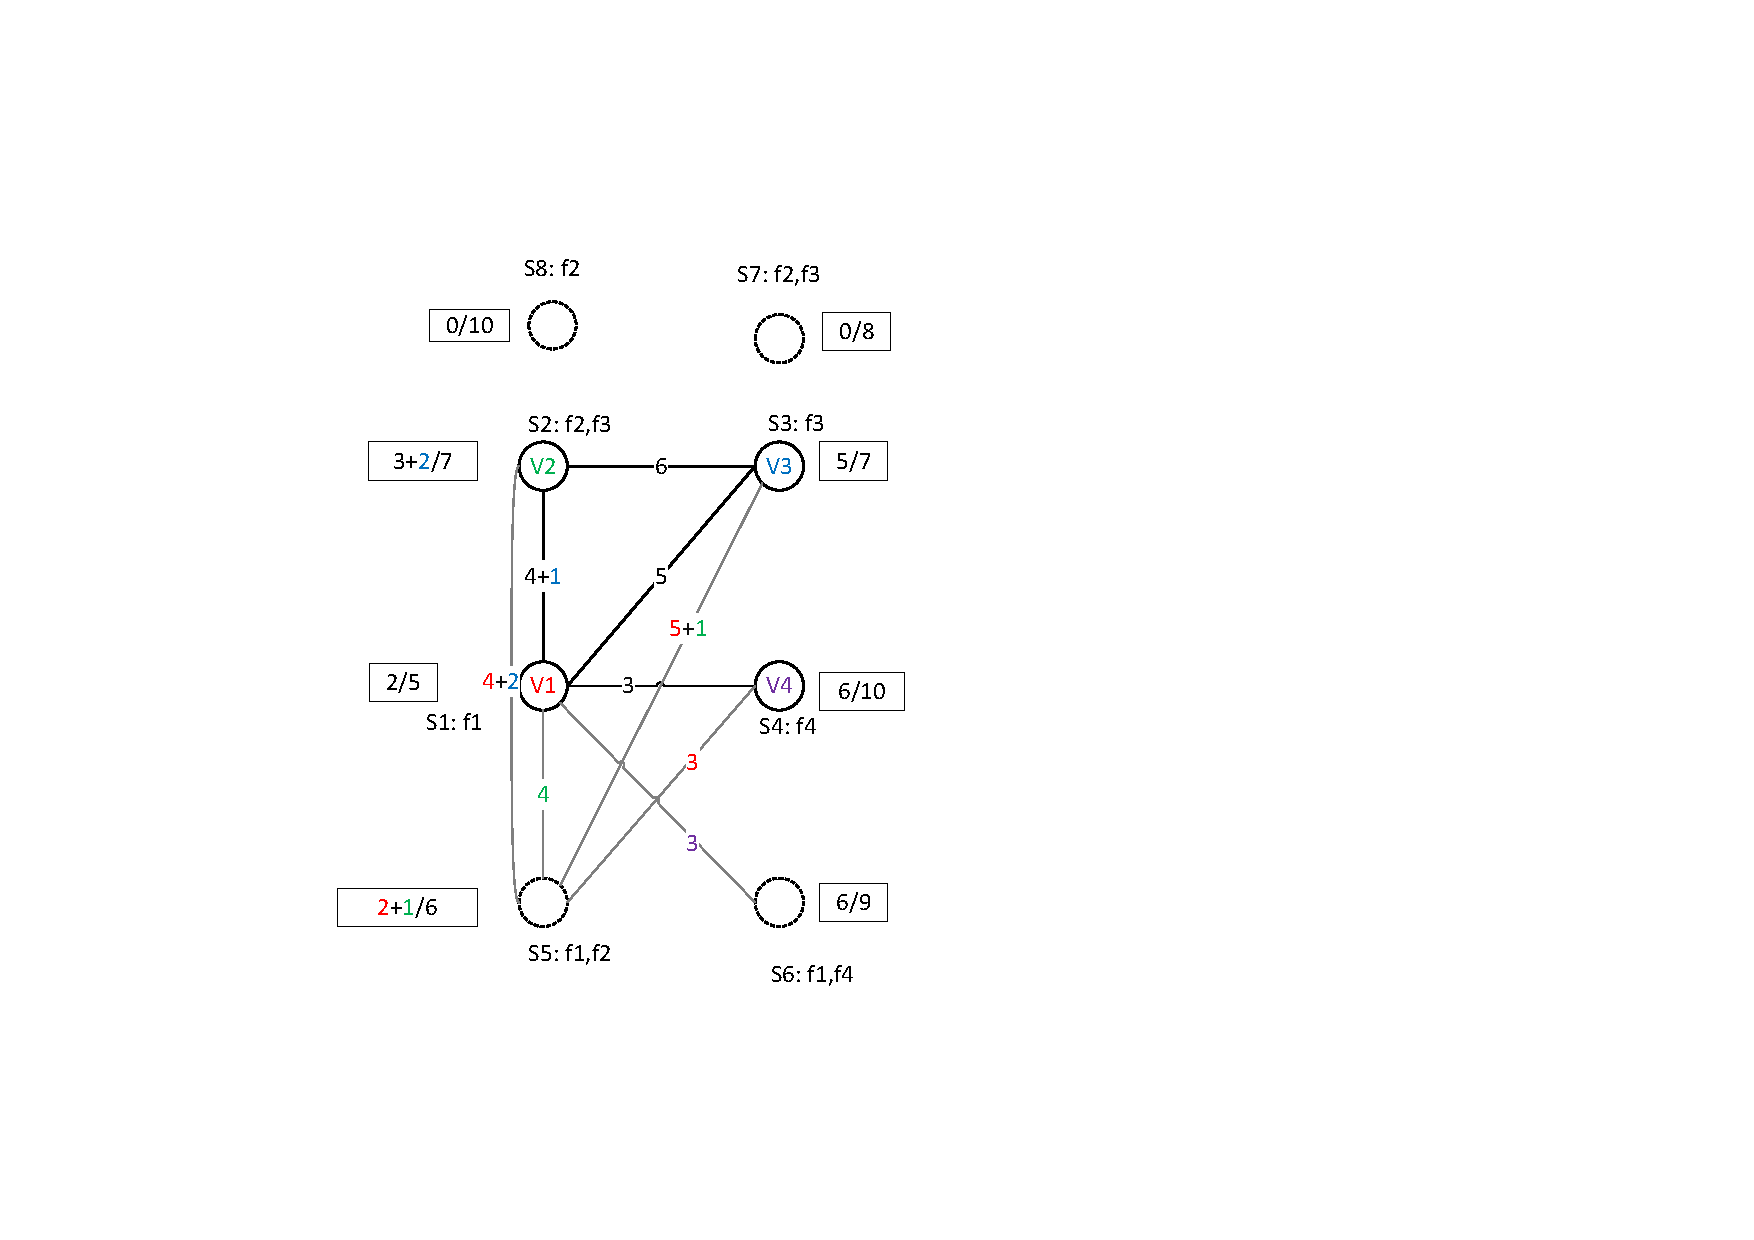
\includegraphics[width=1.5in]{Fig/FD}\\
\caption{ FD}\label{fig:FD}
\end{minipage}
\hfill
\begin{minipage}[t]{0.4\linewidth}
\centering
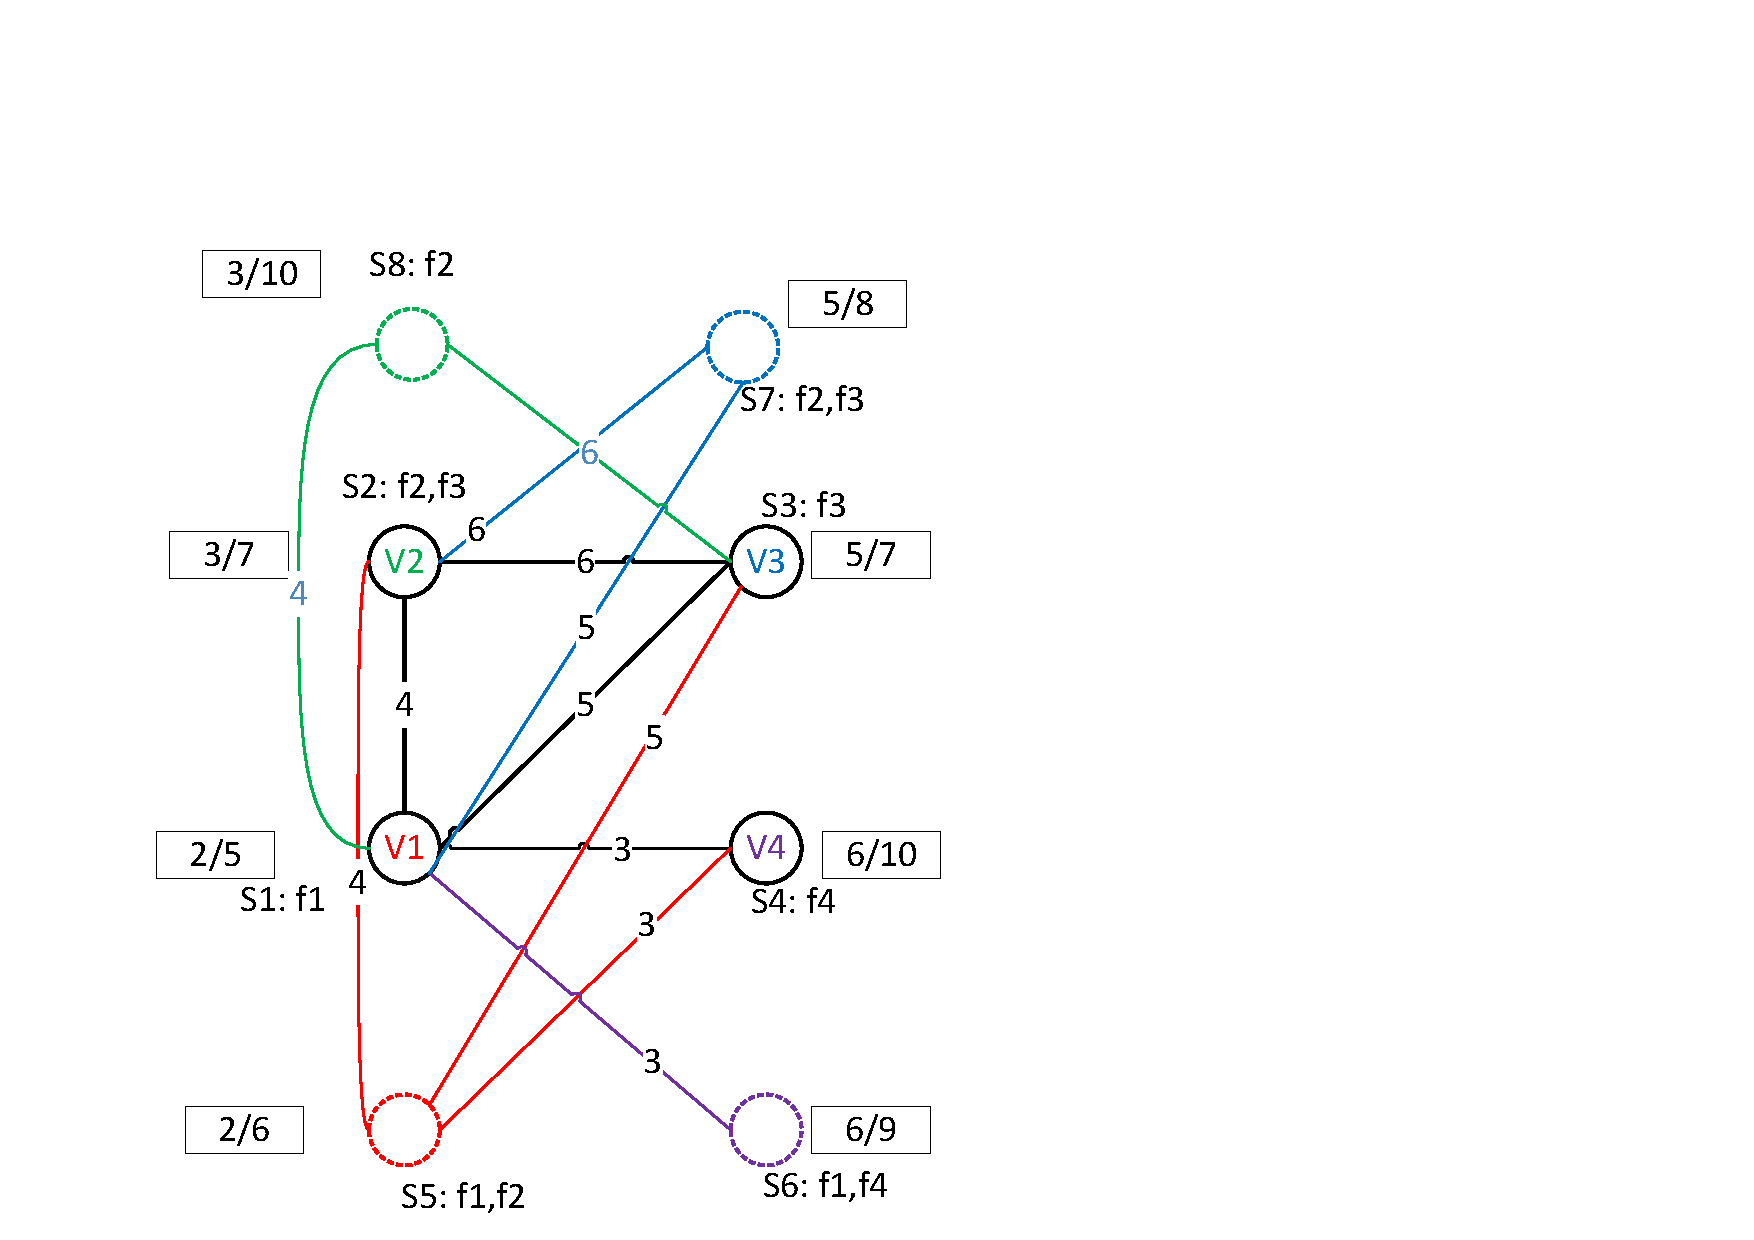
\includegraphics[width=1.5in]{Fig/FI}\\
\caption{1 + 1-protection scheme}\label{fig:FI}
\end{minipage}
\end{figure}




